\chapter{NATURAL RESOURCES}

    \section{VNU-HCM Quarry and Environmental Restoration Efforts}

        \hspace*{0.6cm}Vietnam National University, Ho Chi Minh City (VNU-HCM), manages the Ho Da Quarry Complex—locally known as the ``Lake of Stones''—a legacy of limestone and andesite extraction that supplied construction materials for Saigon's post-war urban expansion from the 1960s to the early 1990s. Situated on elevated terrain within the Linh Trung campus, Linh Trung Ward, Thu Duc City, Ho Chi Minh City, the site comprises five major pits and one minor basin. The primary depression exceeds 60 meters in depth, with the largest lake covering 30 hectares, while quarry rims rise 25--30 meters above the surrounding landscape, forming a prominent topographic feature visible from central Ho Chi Minh City.
        \begin{figure}[H]
            \centering
            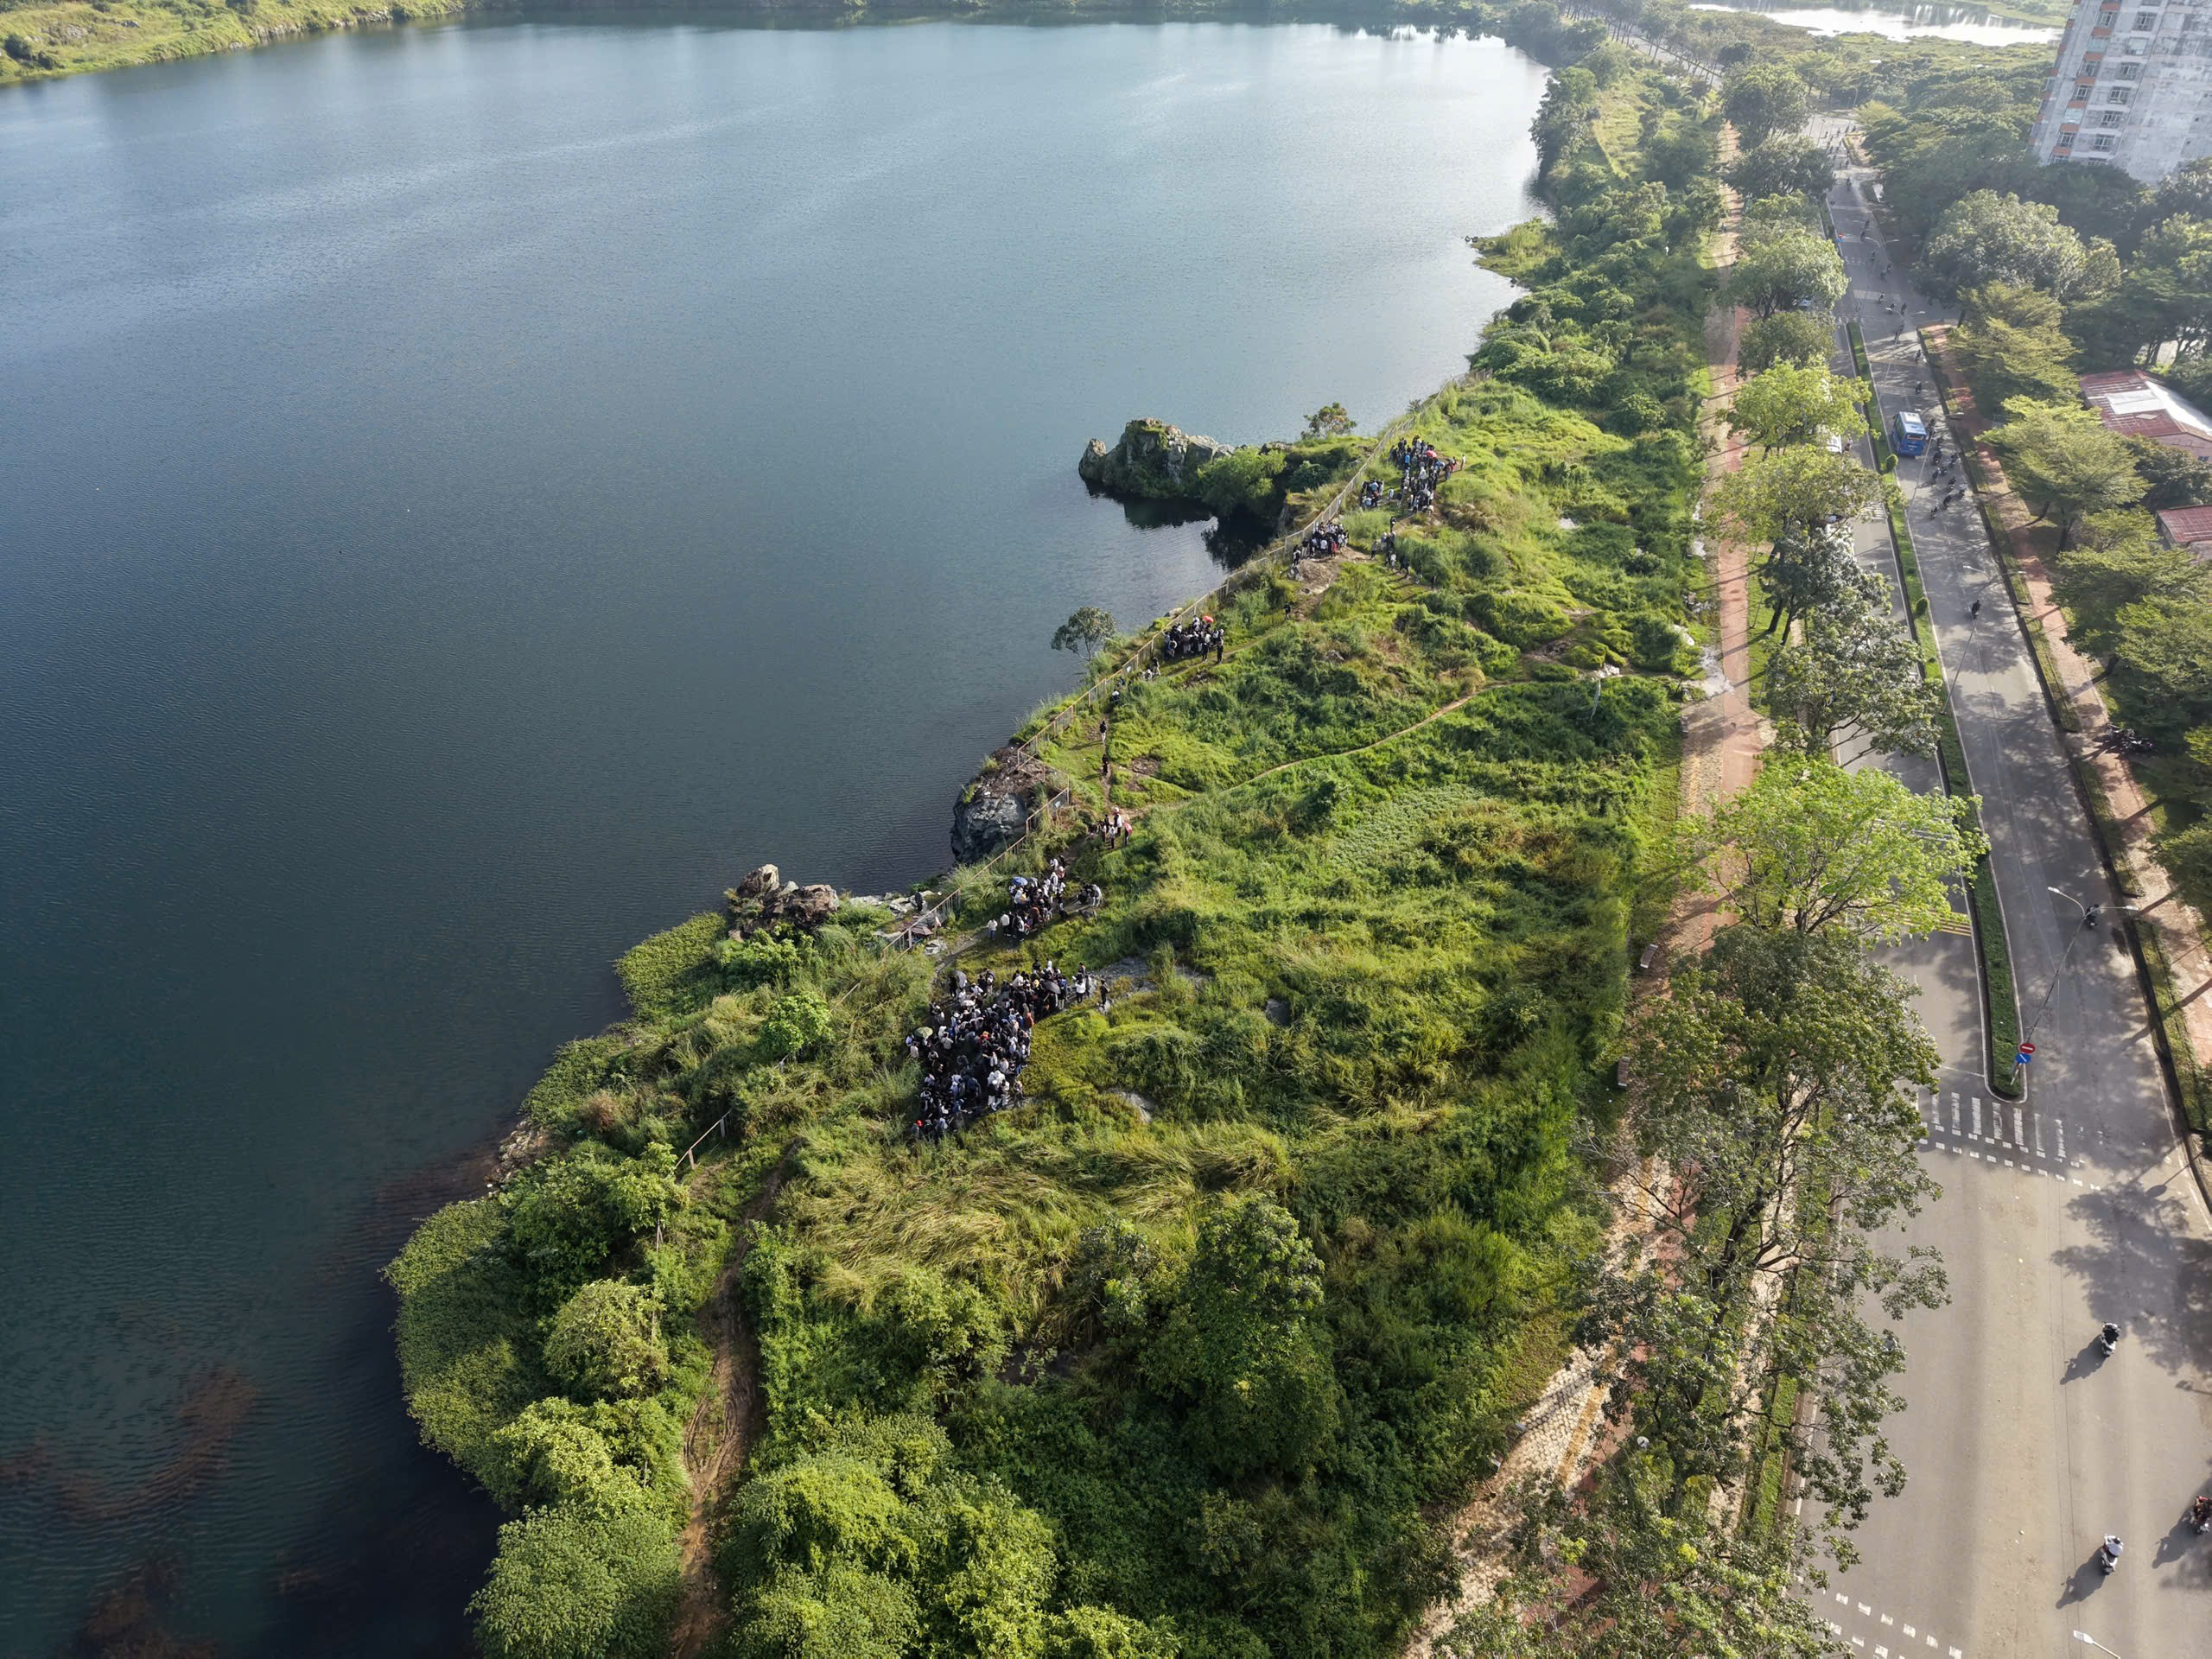
\includegraphics[width=0.7\textwidth]{pictures/chapter5/c5_p1_Lake_of_Stones.png}
            \caption{Aerial view of Ho Da Quarry Complex}
            \label{fig:ho_da_quarry_aerial}
        \end{figure}

        The dominant rock type is andesite, an intermediate volcanic rock (55--62\% SiO$_2$) emplaced during Cretaceous magmatic activity approximately 20 million years ago. Fresh specimens display light gray coloration with a microcrystalline texture (hyalopilitic to intersertal), featuring phenocrysts of andesine plagioclase and minor hornblende in a glassy to microlitic groundmass. Weathered surfaces darken to medium gray due to oxidation of mafic minerals. The rock's blocky jointing and high compressive strength ($>$150 MPa) made it ideal for crushed aggregate (stone chips) and dimension stone (blocks), which were subsequently milled, mixed with binders, and pressed into construction bricks.

        Quarrying severed Cretaceous aquifers, causing rapid pit inundation and abandonment without formal reclamation by 1993. This disruption resulted in a 2.5--4 meter groundwater drawdown over two decades (VNU-HCM Institute of Environment and Resources, 2022), affecting more than 50 local wells within a 3 km radius. Ecological damage included near-total denudation of secondary forest, leaving $<$5\% of the area capable of natural regeneration. Exposed andesite faces accelerated weathering, triggering 12 minor landslides and 3 major collapses between 2000 and 2023. Water-quality monitoring in 2024 (Ho Chi Minh City Environmental Monitoring Center) revealed iron (Fe) and manganese (Mn) levels exceeding QCVN 08:2021/BTNMT by factors of 3.2 and 2.8, respectively, due to prolonged sulfide oxidation under submerged conditions. The site remains a public safety hazard, with at least eight drowning fatalities since 1998 linked to steep drop-offs and hypothermic waters below 18 °C.

        Since 2018, the Ho Da Ecological Restoration Programme (2018--2030)—budgeted at VND 28 billion—has implemented four integrated components. Safety enhancements include 2.2 km of steel fencing, 45 multilingual warning signs, and 12 AI motion-detection cameras, achieving zero drowning incidents since 2020. Geotechnical stabilization uses shotcrete anchoring and vetiver grass across 15,000 m$^2$, reducing annual soil loss by 87\%. Automated monitoring has documented a 42\% decline in average Fe/Mn concentrations. Ecological recovery involves planting 12,000 native trees (\textit{Dipterocarpus alatus}, \textit{Sindora siamensis}, \textit{Melaleuca cajuputi}) and releasing 50,000 fish fingerlings, increasing vegetative cover from 5\% to 35\%. By 2035, the site will transition into an Urban Geo-Ecological Park, integrating education, research, and controlled tourism while preserving andesite outcrops as geological teaching resources.

    \section{Basalt Quarry at Nui Dat -- Dat Do District, Ba Ria -- Vung Tau Province}

        \hspace*{0.6cm}The Nui Dat Basalt Quarry in Dat Do District, Ba Ria--Vung Tau Province, operated from the 1970s until permanent closure in 2005, supplying high-strength aggregate for major infrastructure including the Cai Mep--Thi Vai port complex and the Ho Chi Minh City--Long Thanh--Dau Giay Expressway. Provincial records estimate extraction exceeding 50 million cubic meters across $>$120 hectares, leaving pits 30--50 meters deep and fundamentally altering local topography.
        The bedrock is primary effusive basalt (45--52\% SiO$_2$), erupted as low-viscosity magma that cooled rapidly near the surface to form lava flows and columnar jointing. Coastal zones cooled quickly, producing fine fractures and small columns; inland areas cooled more slowly, forming hexagonal prisms up to 1.5 meters in diameter. Fresh basalt is dark gray to black with aphanitic to porphyritic texture, containing olivine and pyroxene phenocrysts in a plagioclase-rich groundmass. Weathered surfaces develop reddish-brown lateritic crusts due to iron oxidation. Vesicular zones and vitric margins indicate gas exsolution during emplacement. The basalt is unconformably overlain by laterite (bauxitic soil), clearly marking stratigraphic boundaries. Quarrying employed differential blasting to leverage the rock's $>$200 MPa compressive strength and low natural fracturing, minimizing waste.

        Uncontrolled operations caused severe environmental degradation. Erosion rates reached 120 tonnes/ha/year—15 times background levels—resulting in downstream sedimentation that buried $>$15 hectares of agricultural land (Dat Do District, 2018). Vegetation loss exceeded 85\%, and large fauna were displaced. PM$_{10}$ dust during peak operations (1995--2005) exceeded standards by 5--7 times, affecting $>$8,000 residents in adjacent communes. The site's role as a Vietnam War revolutionary base with intact tunnel systems prompted Decision No. 125/QD-UBND (2005) mandating closure.

        The ``Nui Dat Green -- Green Heritage'' initiative implemented a three-phase recovery model. Phase 1 (2006--2010) established 60\% canopy cover using \textit{Acacia mangium} hybrids and \textit{Pinus caribaea}. Phase 2 (2011--2020) allowed natural succession, restoring 40 native plant species. Phase 3 (2021--present) introduced interpretive trails, war relic exhibits, and guided tours, attracting 65,000 visitors annually (Ba Ria--Vung Tau Tourism Department, 2024). Nui Dat now exemplifies integrated restoration, combining geological education (columnar basalt exposures), ecological recovery, and cultural heritage preservation.

    \section{Petroleum Service Industry in Vung Tau (Vietsovpetro Joint Venture)}

        \hspace*{0.6cm}Established on June 19, 1981, under a Vietnam--Soviet bilateral agreement, the Vietsovpetro Joint Venture stands as Vietnam's flagship offshore oil and gas operator. Based in Vung Tau, the company oversees a complete operational cycle—from exploration and drilling to field development, engineering, platform installation, production, and crude oil export—primarily within Block 09-1 (Bach Ho, Rong, and Dai Hung fields), located 120--180 km offshore. By October 2024, Vietsovpetro had achieved a cumulative production of 250 million tonnes of crude oil, generating approximately USD 150 billion in export revenue and consistently accounting for 58--62\% of Vietnam's total national oil output over four decades.
        \begin{figure}[H]
            \centering
            \includegraphics[width=1\textwidth]{pictures/chapter5/c5_p2_Víetsovpetro.png}
            \caption{Some models at Vietsovpetro's showroom}
            \label{fig:vietsovpetro_platform}
        \end{figure}
        The scale of operations is immense, supported by 12 fixed production platforms, 5 self-elevating drilling rigs, and over 420 km of subsea pipelines. A standout asset is the ThTC-02 (Tam Dao 02) rig, capable of drilling 28 wells per dry season to depths of 9,000 meters. Technological innovation is a cornerstone: CO$_2$-enhanced oil recovery (EOR) implemented at the Bach Ho field has increased recovery rates from 35\% to 48\%, a breakthrough protected by multiple patents. Economically, Vietsovpetro has contributed more than USD 65 billion to the state budget from 1981 to 2024, directly employs 8,500 highly skilled workers, and has trained over 15,000 petroleum engineers through partnerships with the Vietnam Petroleum Institute. The company holds 1,826 registered patents, averaging 43 per year.

        Since 2005, Vietsovpetro has diversified beyond production into third-party technical services, providing drilling support for Petronas in Malaysia, platform installation for ExxonMobil's Ca Voi Xanh project, and subsea maintenance in Russia, Algeria, and Venezuela. This expansion has elevated its global technical reputation while reinforcing Vietnam's position in the international energy services market.

        Vietsovpetro maintains a grand exhibition hall and conference center at its Vung Tau headquarters, a vast, modern facility designed to showcase four decades of industrial achievement and technological prowess. The expansive space features full-scale equipment replicas, interactive scale models of offshore platforms and rigs, core samples from deep reservoirs, historical drilling tools, early control systems, and an extensive gallery of patents, awards, and operational timelines. The hall serves as both a corporate heritage center and a public education venue, welcoming engineers, students, and international delegations.

        Sustainability is now a strategic priority. Vietsovpetro operates a zero-discharge water treatment system that recycles 97\% of produced water, preventing marine contamination. Between 2018 and 2024, the company reduced methane emissions by 42\% through flare gas recovery and advanced leak detection (Vietsovpetro Sustainability Report 2023). A 400 MW offshore wind farm within Block 09-1 received investment approval in 2024, with construction set to begin in 2026. Looking forward, Vietsovpetro aims to maintain crude output at 5--6 million tonnes annually through 2035 while redirecting 30\% of revenue toward green energy initiatives, including carbon capture and storage (CCS), blue hydrogen production, and renewable integration—positioning the company as a bridge between Vietnam's hydrocarbon legacy and its net-zero future.

        In contrast to the andesite of Ho Da and the basalt of Nui Dat—both volcanic rocks used for construction—Vietsovpetro exploits Miocene clastic reservoirs in the Cuu Long Basin. These consist of turbidite sandstones trapping light-to-medium crude (API gravity 30--40°, sulfur $<$0.5\%) sourced from lacustrine Oligocene shales. This geological shift underscores Vietnam's diverse natural resource portfolio, spanning igneous building materials to sedimentary energy reserves.